\section{Hardware necesario e instalación}

Para crear este sistema de seguridad se necesitan los siguientes componentes:

\begin{figure}[h]
	\centering
	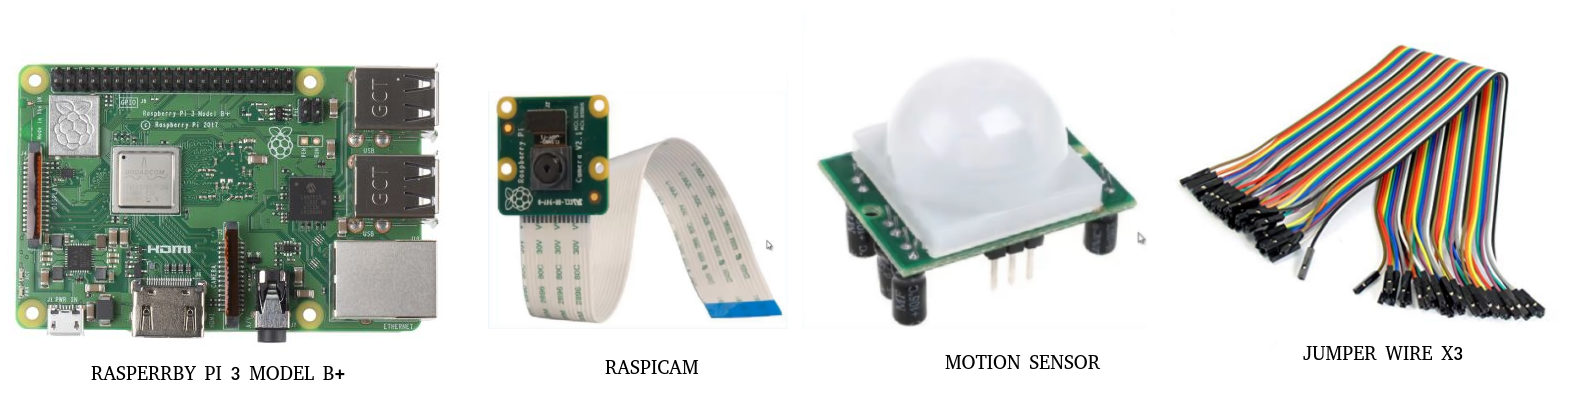
\includegraphics[scale=0.35]{images/44}
	\caption{Componentes hardware sistema de seguridad}
\end{figure}

Cuando hablamos de Raspberry PI, nos referimos al conjunto de elementos necesarios para que funcione (normalmente, siempre se incluye en un paquete), como son la fuente de alimentación y la tarjeta SD donde hemos instalado un SO (en este caso Raspbian 9).

\textbf{Guía de instalación de hardware}

\begin{itemize}

\item  En primer lugar, hay que conectar el módulo de la cámara a la Raspberry PI. Para ello se instala el módulo Raspberry Pi Camera insertando el cable en la Raspberry PI. El cable se encaja en el conector situado entre los puertos Ethernet y HDMI, con los conectores plateados orientados hacia el puerto HDMI, tal y como se muestra en la siguiente imagen.


\begin{figure}[H]
	\centering
	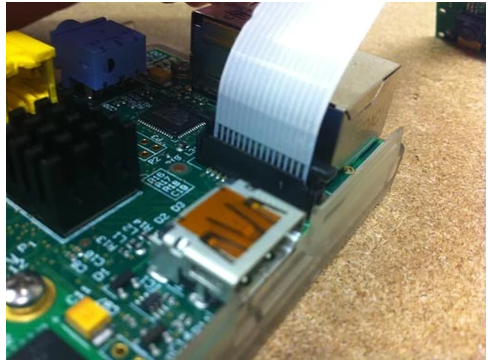
\includegraphics[scale=0.45]{images/46}
	\caption{Conexión del módulo de la cámara a la Raspberry PI}
\end{figure}

\item Enciende la Raspberry PI y desde el prompt, ejecute:

\vspace{-1cm}

\begin{verbatim}

# sudo raspi-config

\end{verbatim}

\vspace{-1cm}

Si la opción `cámara' no aparece en la lista, entonces es necesario ejecutar una serie de comandos para poder actualizar la Raspberry PI. Para realizar esto, puede ejecutar lo siguiente:

\vspace{-1cm}

\begin{verbatim}

# sudo apt-get update && sudo apt-get upgrade

\end{verbatim}

\vspace{-1cm}

\item Ahora sí, deberá de aparecer la opción para la cámara al ejecutar \texttt{sudo raspi-config}.

\begin{figure}[H]
	\centering
	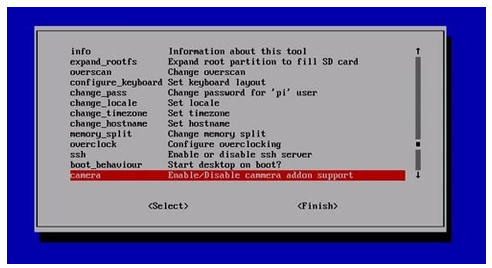
\includegraphics[scale=0.9]{images/47}
	\caption{Activación de la cámara en la Raspberry PI}
\end{figure}

\vspace{-0.4cm}

\item Una vez que haya instalado la cámara y comprobado que funciona, el siguiente paso es instalar el sensor de movimiento. Para ello tenemos que conectar los cables de puente como se indica en la siguiente figura (preste atención a los colores que indican dónde se ha conectado cada clavija).

\begin{figure}[H]
	\centering
	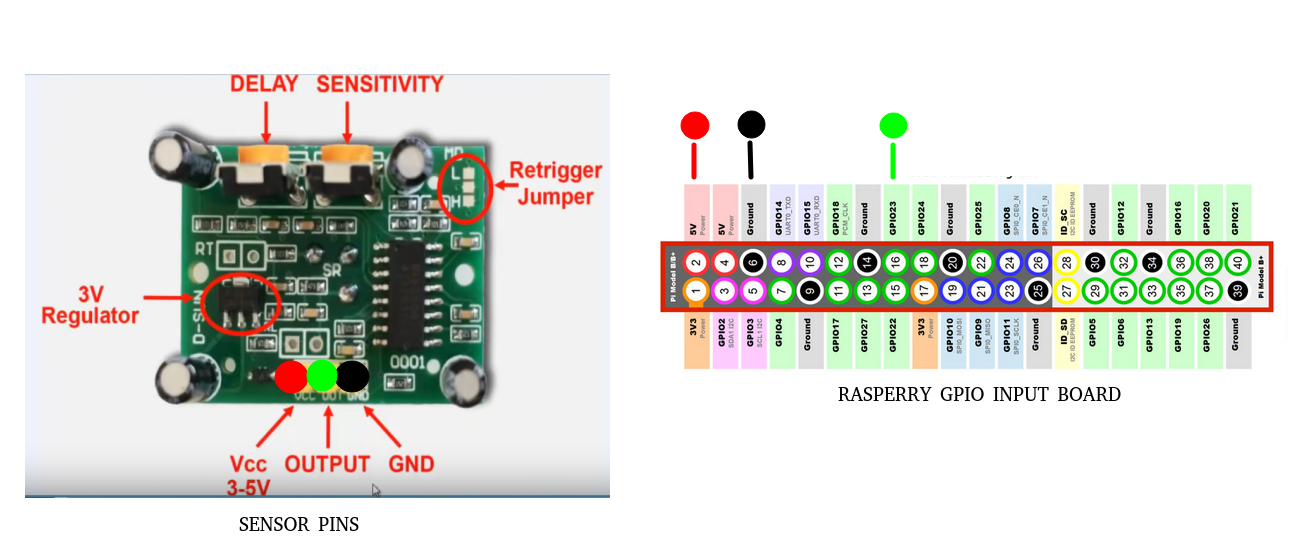
\includegraphics[scale=0.37]{images/48}
	\caption{Activación de la cámara en la Raspberry PI}
\end{figure}

\item Intenta sujetar bien los componentes y colocar la Raspberry PI junto con el sensor de movimiento en la zona que desee vigilar. Por ejemplo:

\begin{figure}[H]
	\centering
	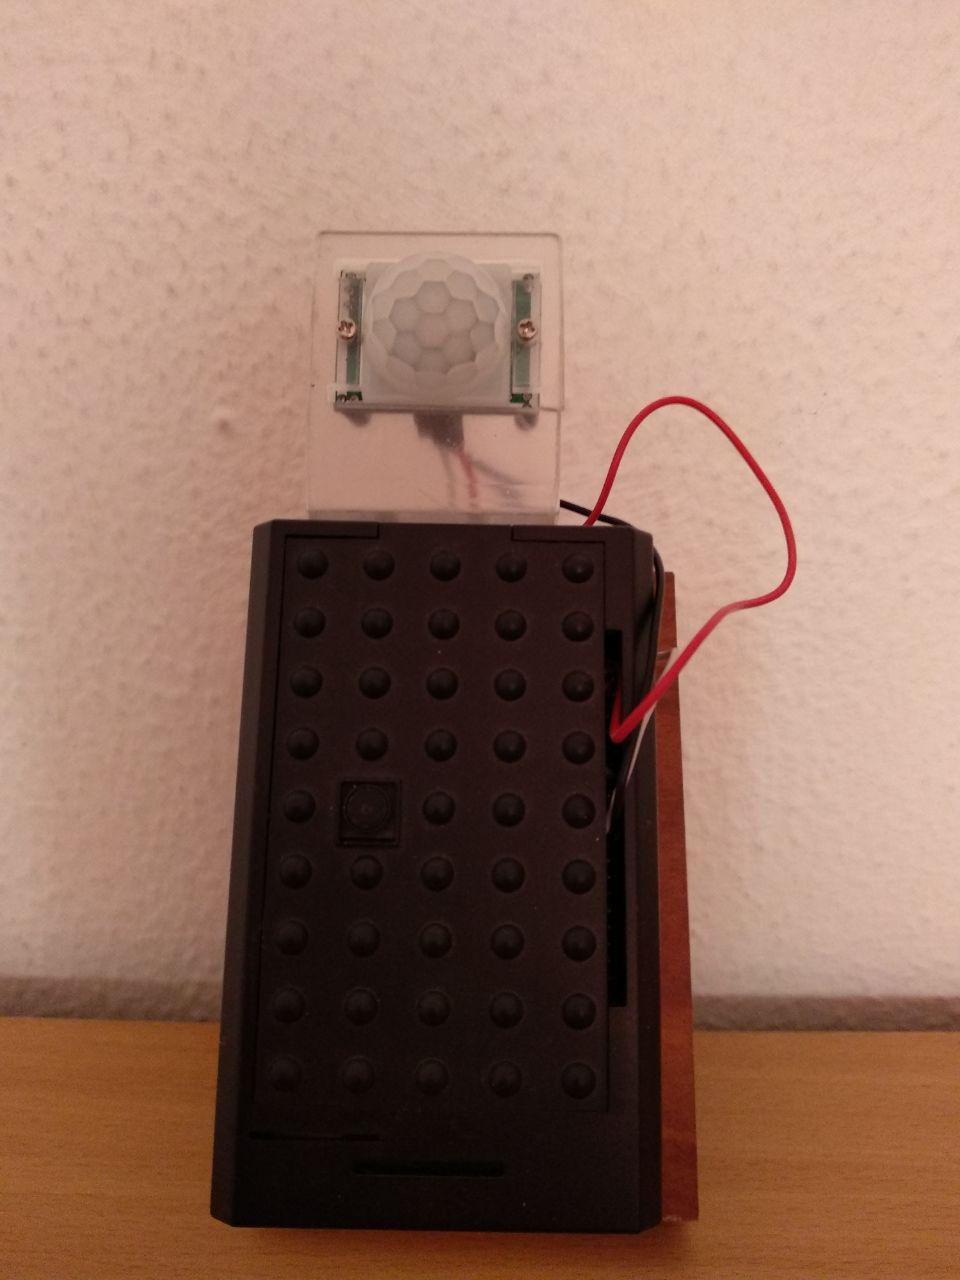
\includegraphics[scale=0.23]{images/56}
	\caption{Raspberry PI conectada a la cámara y al sensor de movimiento}
\end{figure}

\end{itemize}

\textbf{Compra de los componentes}

A continuación se presentan los componentes que se han utilizado para desarrollar este proyecto y un enlace de compra:

\begin{itemize}
\item Paquete de iniciación. Precio: 50.66\euro.  \href{https://es.aliexpress.com/item/32919276764.html?spm=a2g0o.productlist.0.0.68c17409mViI9v&s=p&algo_pvid=3b970bb1-7255-4a8b-a98d-624a8c9b16c7&algo_expid=3b970bb1-7255-4a8b-a98d-624a8c9b16c7-1&btsid=cb6fa330-c76b-4821-ae48-adb8325769c2&ws_ab_test=searchweb0_0,searchweb201602_10,searchweb201603_53}{Enlace de compra}.

\begin{figure}[H]
	\centering
	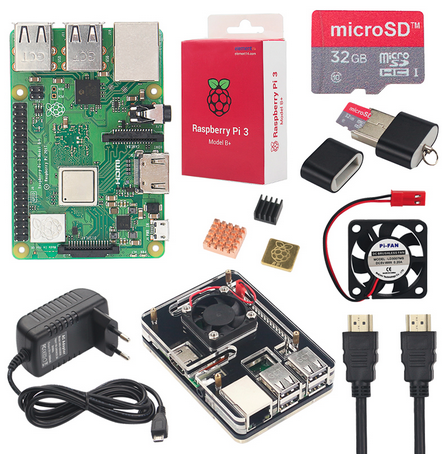
\includegraphics[scale=0.4]{images/50}
	\caption{Pack básico de la Raspberry PI y sus componentes}
\end{figure}

\newpage

\item Caja de la Raspberry PI con soporte para la cámara. Precio: 10.69\euro. \href{https://es.aliexpress.com/item/32672860034.html?spm=a2g0s.9042311.0.0.683c63c0C8GUcZ}{Enlace de compra}.

\begin{figure}[H]
	\centering
	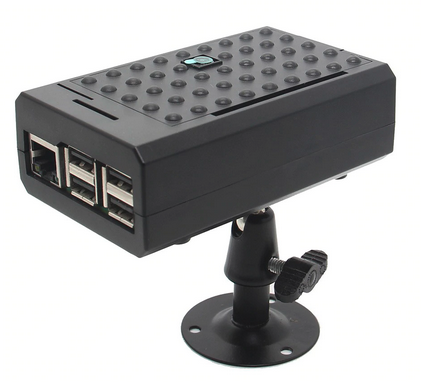
\includegraphics[scale=0.4]{images/51}
	\caption{Caja con soporte de cámara para Raspberry PI}
\end{figure}

\item Sensores de movimiento y soporte. Precio: 1\euro. \href{https://es.aliexpress.com/item/32731348914.html?spm=a2g0s.9042311.0.0.114163c0wdGfJC}{Enlace de compra}.

\begin{figure}[H]
	\centering
	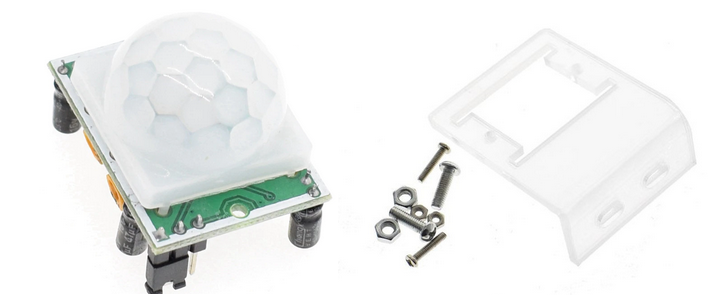
\includegraphics[scale=0.4]{images/52}
	\caption{Sensores de movimiento y soporte}
\end{figure}

\item Módulo de cámara para Raspberry PI. Precio: 5.8\euro. \href{https://es.aliexpress.com/item/32968556678.html?spm=a2g0o.productlist.0.0.279c19a8naSYJL&algo_pvid=5214796b-f890-4536-bfe3-6dfdd7068ebe&algo_expid=5214796b-f890-4536-bfe3-6dfdd7068ebe-20&btsid=d3f277b6-2fe7-4e0e-b9c1-9190cc1ac969&ws_ab_test=searchweb0_0,searchweb201602_10,searchweb201603_53}{Enlace de compra}.

\begin{figure}[H]
	\centering
	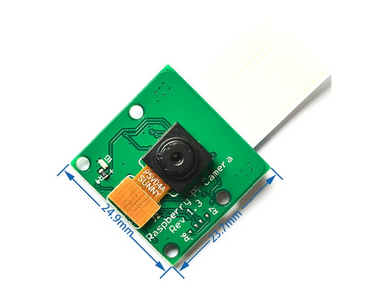
\includegraphics[scale=0.4]{images/53}
	\caption{Módulo de cámara para Raspberry PI}
\end{figure}

\newpage

\item Cables jumper. Precio: 2.48\euro. \href{https://es.aliexpress.com/item/32964957576.html?spm=a2g0o.productlist.0.0.61d17325XdrqJt&algo_pvid=47c5409e-0ddd-4fcc-8cb6-9ecadcd35c74&algo_expid=47c5409e-0ddd-4fcc-8cb6-9ecadcd35c74-3&btsid=db357dd3-7316-46fa-b765-64d122cc0043&ws_ab_test=searchweb0_0,searchweb201602_10,searchweb201603_53}{Enlace de compra}.

\begin{figure}[H]
	\centering
	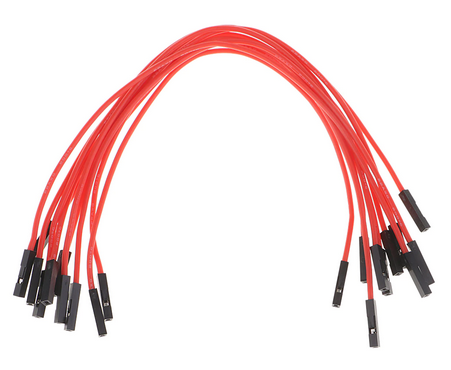
\includegraphics[scale=0.4]{images/54}
	\caption{Cables jumper para conectar el sensor de movimiento a la placa de PINS}
\end{figure}


\end{itemize}